% Rapport du projet SdF — version LaTeX générée par report/build.mjs --latex (ne pas modifier à la main :
% modifier report/source/*.md puis régénérer). Compiler de préférence avec XeLaTeX (latexmk lit .latexmkrc) ;
% pdfLaTeX (défaut d'Overleaf) fonctionne aussi : le résumé arabe est alors inclus en image.
\documentclass[12pt,a4paper,oneside]{report}

% ---------- polices et langues ----------
\usepackage{iftex}
\usepackage{amsmath}
\ifXeTeX
  \usepackage{mathptmx}
  \usepackage{fontspec}
  % Times New Roman si elle est installée, sinon son clone libre TeX Gyre Termes, désigné par ses fichiers
  % (trouvés par TeX Live partout, Overleaf compris, même quand la police n'est pas déclarée au système)
  \IfFontExistsTF{Times New Roman}{\setmainfont{Times New Roman}}
    {\IfFontExistsTF{TeX Gyre Termes}{\setmainfont{TeX Gyre Termes}}
      {\setmainfont{texgyretermes}[Extension=.otf,UprightFont=*-regular,BoldFont=*-bold,ItalicFont=*-italic,BoldItalicFont=*-bolditalic]}}
  \setmonofont{lmmono10-regular}[Extension=.otf,Scale=0.95]
  \usepackage[bidi=default,english,french]{babel}
  \frenchsetup{StandardLists=true,SmallCapsFigTabCaptions=false}
  \babelprovide[import]{arabic}
  \babelfont[arabic]{rm}[Scale=1.15]{Amiri}
  \newcommand{\arabicabstract}{\begin{otherlanguage}{arabic}% généré depuis source/15_resumes.md
\noindent{\large\bfseries ملخص}\par\medskip


يقدّم هذا التقرير دراسة في سلامة التشغيل والصيانة التنبّؤية أُجريت على مجموعة البيانات العمومية NASA C-MAPSS FD001، التي تحاكي تدهور المحرّكات التوربينية النفّاثة حتى العطل. يعالج تحليل الموثوقية 100 محرّكًا ما زالت في الخدمة باعتبارها مُدَدًا مبتورة من اليمين، ويعتمد قانون فايبل ذا المعاملات الثلاثة الذي قَبِله اختبار كولموغوروف-سميرنوف، ويبلغ متوسّط مدّة التشغيل قبل العطل 206,3 دورة. ووفق فرضيات إصلاح مُصرَّح بها، تبلغ الإتاحة الذاتية 95,98 \%، ويُخفّض الاستبدال الوقائي عند عمر 131 دورة كلفة الدورة بنسبة 68 \%. وتبني سلسلة الصيانة التنبّؤية مؤشّرًا للحالة الصحّية انطلاقًا من 12 حسّاسًا، وتكشف الحالة الحرجة بمساحة تحت المنحنى قدرها 0,991، وتقدّر العمر المتبقّي بنموذج تدهور بايزي (جذر متوسّط مربّع الخطأ 24,47 دورة) وبشبكة LSTM (جذر متوسّط مربّع الخطأ 15,35 دورة). وكلّ رقم في هذا التقرير ناتج عن الشيفرة ومُتحقَّق منه باختبارات آلية.


\textbf{الكلمات المفاتيح:} الموثوقية، البتر من اليمين، قانون فايبل، الإتاحة، الصيانة التنبّؤية، العمر المتبقّي.
\end{otherlanguage}}
\else
  \usepackage[T1]{fontenc}
  \usepackage[utf8]{inputenc}
  \usepackage{mathptmx}
  \usepackage[scaled=0.92]{helvet}
  \usepackage{lmodern}\renewcommand{\rmdefault}{ptm}\renewcommand{\ttdefault}{lmtt}
  \usepackage[english,french]{babel}
  \frenchsetup{StandardLists=true,SmallCapsFigTabCaptions=false}
  \newcommand{\arabicabstract}{\noindent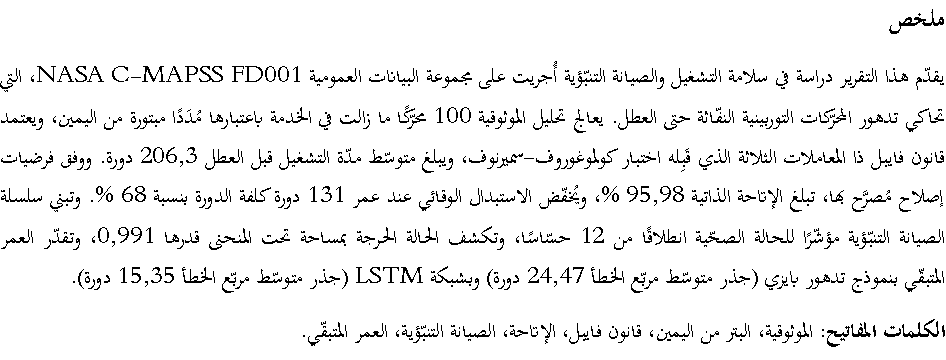
\includegraphics[width=\linewidth]{figures/resume_arabe.pdf}}
\fi

% ---------- mise en page ----------
\usepackage[a4paper,top=2.6cm,bottom=2.6cm,left=2.5cm,right=2.5cm,headheight=15pt]{geometry}
\usepackage{setspace}\setstretch{1.3}
\setlength{\parindent}{0pt}
\setlength{\parskip}{4pt}
\usepackage{xcolor}
\definecolor{navy}{RGB}{20,30,110}
\definecolor{linkblue}{RGB}{28,84,140}
\definecolor{headgray}{RGB}{90,90,90}
\definecolor{boxgray}{RGB}{244,244,244}

\usepackage{titlesec}
\titleformat{\chapter}[display]{\normalfont\bfseries\fontsize{26}{30}\selectfont}
  {\chaptertitlename\ \thechapter}{14pt}{\fontsize{24}{28}\selectfont}
\titlespacing*{\chapter}{0pt}{20pt}{24pt}
\titleformat{name=\chapter,numberless}[display]{\normalfont\bfseries\fontsize{26}{30}\selectfont}{}{0pt}{}
\titlespacing*{name=\chapter,numberless}{0pt}{20pt}{24pt}
\titleformat{\section}{\normalfont\Large\bfseries\color{headgray}}{\thesection}{0.8em}{}
\titleformat{\subsection}{\normalfont\large\bfseries\color{headgray}}{\thesubsection}{0.8em}{}

\usepackage{fancyhdr}
\pagestyle{fancy}\fancyhf{}
\fancyhead[L]{\small\color{headgray}FMDS et maintenance prédictive}
\fancyhead[R]{\small\color{headgray}\nouppercase{\leftmark}}
\fancyfoot[C]{\thepage}
\renewcommand{\headrulewidth}{0.5pt}
\renewcommand{\chaptermark}[1]{\markboth{\chaptername\ \thechapter.\ #1}{}}
\fancypagestyle{plain}{\fancyhf{}\fancyfoot[C]{\thepage}\renewcommand{\headrulewidth}{0pt}}
\newcommand{\frontmark}[1]{\markboth{#1}{#1}}

% ---------- contenu ----------
\usepackage{graphicx}
\usepackage{booktabs,tabularx,array}
\usepackage{adjustbox}
\usepackage{amssymb}
\usepackage{enumitem}\setlist{itemsep=2pt,topsep=4pt}\setlist[itemize]{label=\textbullet}
\usepackage{caption}\captionsetup{labelsep=colon,font=normalsize,skip=8pt}
\usepackage{float}
\usepackage{multicol}
\usepackage[most]{tcolorbox}
\usepackage[hidelinks,colorlinks=true,linkcolor=linkblue,citecolor=teal,urlcolor=linkblue]{hyperref}

\newcommand{\codeus}{\textunderscore\allowbreak}
\newcommand{\code}[1]{{\ttfamily\let\_\codeus #1}}
\newtcolorbox{problembox}{colback=boxgray,colframe=boxgray,boxrule=0pt,arc=0pt,
  left=10pt,right=10pt,top=8pt,bottom=8pt,fontupper=\itshape,halign=center}

% Introduction / Conclusion non numérotées dans chaque chapitre
\newcommand{\chapintro}{\section*{Introduction}}
\newcommand{\chapconclusion}{\section*{Conclusion}}

\addto\captionsfrench{\renewcommand{\listfigurename}{Liste des figures}\renewcommand{\listtablename}{Liste des tableaux}%
  \renewcommand{\tablename}{Tableau}%
  \renewcommand{\contentsname}{Table des matières}\renewcommand{\bibname}{Bibliographie}}

\setcounter{tocdepth}{1}

\begin{document}
% généré depuis source/00_titre.md — ne pas modifier à la main
% =================== PAGE DE GARDE ===================
\begin{titlepage}
\newgeometry{top=1.4cm,bottom=1.6cm,left=2.4cm,right=2.4cm}
\setstretch{1.05}
\centering
\noindent
\begin{minipage}[c]{0.3\linewidth}\raggedright
  \IfFileExists{figures/logo_univ_tunis.png}{
\includegraphics[height=2.1cm,keepaspectratio]{figures/logo_univ_tunis.png}}{}
\end{minipage}%
\begin{minipage}[c]{0.4\linewidth}\centering
  
\includegraphics[height=2.2cm,keepaspectratio]{figures/logo_emblem.png}
\end{minipage}%
\begin{minipage}[c]{0.3\linewidth}\raggedleft
  
\includegraphics[height=1.5cm,keepaspectratio]{figures/logo_ensit.png}
\end{minipage}

\vspace{0.5cm}
{\color{navy}\rule{\linewidth}{1pt}}\par
\vspace{0.35cm}
{\large\bfseries UNIVERSITÉ DE TUNIS\par}
\vspace{2pt}
{\large\bfseries ÉCOLE NATIONALE SUPÉRIEURE D'INGÉNIEURS DE TUNIS\par}
\vspace{2pt}
{\bfseries DÉPARTEMENT DE GÉNIE MATHÉMATIQUE\par}
\vspace{0.3cm}
{\color{navy}\rule{\linewidth}{1pt}}\par

\vspace{0.7cm}
{\LARGE\bfseries Projet de Sûreté de Fonctionnement et Maintenance\par}
\vspace{0.3em}
{\large\bfseries Troisième année — Génie Mathématiques Appliquées et Modélisation (GMAM 3)\par}

\vspace{0.7cm}
{\normalsize Présenté par\par}
\vspace{0.4em}
{\LARGE\bfseries Eya DHRIF\\[0.2em] Salma MOUEDDEB\par}

\vspace{0.7cm}
\rule{0.85\linewidth}{0.6pt}\par
\vspace{0.6em}
{\fontsize{22}{27}\selectfont\bfseries\color{navy} Estimation des indices FMDS et maintenance prédictive\par}
\vspace{0.35em}
{\Large\bfseries d'une flotte de turboréacteurs simulés (NASA C-MAPSS FD001)\par}
\vspace{0.6em}
\rule{0.85\linewidth}{0.6pt}\par

\vspace{0.6cm}
{\normalsize Rapport scientifique — Version 1\par}
\vspace{0.7cm}
{\normalsize\textbf{Encadré par :} M. Fayçal Ben Hmida\par}

\vfill
{\normalsize\textbf{Année universitaire :} 2026–2027\par}

\restoregeometry
\end{titlepage}
% =================== FIN DE LA PAGE DE GARDE ===================



\pagenumbering{arabic}
% généré depuis source/01_front.md — ne pas modifier à la main
\chapter*{Dédicaces}
\addcontentsline{toc}{chapter}{Dédicaces}
\frontmark{Dédicaces}

\vspace*{2.5cm}
\begin{center}
\itshape
À nos parents,\\
pour leur amour, leurs sacrifices\\
et leur soutien constant tout au long de nos études.\\[1.4em]
À nos familles et à nos amis,\\
qui nous ont accompagnées à chaque étape.\\[1.4em]
À nos enseignants,\\
qui ont formé notre manière de raisonner.\\[1.4em]
À toutes celles et à tous ceux qui pensent que la rigueur et la curiosité\\
rendent la technique réellement utile.
\end{center}

\chapter*{Remerciements}
\addcontentsline{toc}{chapter}{Remerciements}
\frontmark{Remerciements}

Au terme de ce projet, nous tenons à exprimer notre sincère gratitude à \textbf{M. Fayçal Ben Hmida}, enseignant du module « Sûreté de fonctionnement et maintenance », pour la qualité de son enseignement, pour la clarté avec laquelle il a présenté la démarche d'estimation des indices FMDS, et pour ses conseils, qui ont orienté à la fois la méthode et la rédaction de ce travail.

Nos remerciements vont également à l'ensemble du corps enseignant de l'École Nationale Supérieure d'Ingénieurs de Tunis (ENSIT), pour la formation qu'il nous apporte et qui a fourni les outils sur lesquels ce projet repose.

Nous remercions aussi le centre de recherche Ames de la NASA, qui met à la disposition de la communauté scientifique le jeu de données C-MAPSS sans lequel cette étude n'aurait pas été possible.

Enfin, nous remercions toutes les personnes qui, directement ou indirectement, par leurs remarques, leurs encouragements et leur soutien, ont contribué à l'aboutissement de ce travail.

% généré depuis source/02_listes.md — ne pas modifier à la main

\tableofcontents

\clearpage\frontmark{Liste des figures}
\listoffigures

\clearpage\frontmark{Liste des tableaux}
\listoftables

\clearpage
\setcounter{page}{1}
% généré depuis source/03_introduction_generale.md — ne pas modifier à la main
\chapter*{Introduction générale}
\addcontentsline{toc}{chapter}{Introduction générale}
\frontmark{Introduction générale}

La maintenance des turboréacteurs pèse lourdement sur le coût d'exploitation d'une flotte aérienne. Une défaillance en service immobilise l'appareil et peut mettre en jeu la sécurité ; un remplacement trop précoce gaspille une partie de la vie utile des composants. Entre ces deux écueils, l'exploitant doit connaître le comportement statistique de sa flotte, ses indices de fiabilité, de maintenabilité et de disponibilité, et, de plus en plus, estimer pour chaque moteur la durée de vie qui lui reste à partir des mesures de ses capteurs.

Ce projet, réalisé en binôme dans le cadre du module « Sûreté de fonctionnement et maintenance », applique cette démarche au jeu de données public NASA C-MAPSS, sous-ensemble FD001, qui simule la dégradation jusqu'à la défaillance de turboréacteurs \cite{saxena2008data,saxena2008damage}. Il répond à la question suivante :

\begin{problembox}
À partir des seules données de capteurs d'une flotte de turboréacteurs, comment quantifier la fiabilité de cette flotte, en déduire une politique de maintenance préventive, puis aller au-delà avec une maintenance prédictive moteur par moteur, en garantissant que chaque résultat est exact, reproductible et justifié ?
\end{problembox}

L'étude suit deux axes complémentaires. Le premier estime les indices FMDS de la flotte, en tenant compte des moteurs encore en service, et en déduit une politique de remplacement préventif. Le second construit une chaîne de maintenance prédictive : indicateur de santé, détection de l'état critique et estimation de la durée de vie résiduelle par deux modèles de natures différentes, un modèle de dégradation bayésien interprétable et un réseau de neurones récurrent. Les résultats sont servis par une API et un tableau de bord web, et chaque chiffre du rapport est produit par le code et vérifié par une suite de tests automatiques.

Le rapport comporte sept chapitres. Le chapitre~\ref{sec:etat-art} pose le cadre du projet et présente un état de l'art ciblé. Le chapitre~\ref{sec:donnees} décrit les données et le chapitre~\ref{sec:methodologie} les méthodes, avec leurs fondements mathématiques et leurs hypothèses. Le chapitre~\ref{sec:architecture} présente l'architecture et la mise en œuvre du système. Le chapitre~\ref{sec:resultats} expose le protocole expérimental et les résultats, discutés au chapitre~\ref{sec:discussion}. Le chapitre~\ref{sec:perspectives} présente les perspectives, avant la conclusion générale.

% généré depuis source/04_cadre_donnees.md — ne pas modifier à la main
\chapter{Cadre du projet, état de l'art et jeu de données}\label{sec:cadre}

\chapintro

Ce chapitre présente le contexte industriel, la problématique et les objectifs du projet, puis un état de l'art ciblé sur les méthodes utilisées. Il décrit enfin le jeu de données C-MAPSS FD001.

\section{Contexte industriel et problématique}\label{sec:contexte}

La norme NF EN 13306 \cite{nf13306} distingue trois familles de maintenance : \textbf{corrective}, après la défaillance ; \textbf{préventive systématique}, à intervalles fixes ; \textbf{conditionnelle et prévisionnelle}, déclenchée par l'état mesuré du bien et par la prévision de son évolution \cite{jardine2006}. Choisir entre elles demande deux connaissances : le comportement statistique de la flotte, décrit par les indices FMDS \cite{benhmida}, et l'état de santé de chaque moteur en service, avec sa RUL \cite{lei2018,si2011}.

La problématique est donc la suivante : à partir des seules données de capteurs de C-MAPSS FD001, comment quantifier la fiabilité de la flotte, en déduire une politique préventive, puis passer à une maintenance prédictive moteur par moteur ?

\section{Objectifs et contributions}\label{sec:objectifs}

Le projet poursuit quatre objectifs : (\textbf{1}) estimer les indices FMDS en tenant compte de la censure des moteurs encore en service ; (\textbf{2}) construire un HI et détecter les moteurs proches de la défaillance ; (\textbf{3}) estimer la RUL par un modèle de dégradation probabiliste et par un réseau récurrent, puis les comparer ; (\textbf{4}) restituer ces résultats dans un tableau de bord web.

Les contributions qui en découlent sont :

\begin{itemize}
\item une analyse de fiabilité avec censure à droite, quatre lois candidates, des tests d'adéquation et le choix argumenté d'une loi de Weibull à trois paramètres ;
\item une étude de maintenabilité et de disponibilité, fondée sur des temps de réparation simulés et signalés comme tels, avec l'optimisation d'un remplacement préventif à âge fixe ;
\item une chaîne prédictive complète : sélection des capteurs, HI, classification de l'état et deux modèles de RUL, dont un modèle bayésien qui fournit une distribution de la RUL ;
\item un diagnostic explicite des limites, en particulier la calibration insuffisante du modèle de dégradation ;
\item un système reproductible dont chaque résultat est vérifié par des tests automatiques.
\end{itemize}

\section{État de l'art ciblé}\label{sec:ea}

\subsection{Indices FMDS}\label{sec:ea-fmds}

La fiabilité $R(t)$ est la probabilité qu'un bien fonctionne sur $[0, t]$, la maintenabilité $M(t)$ celle qu'une réparation soit achevée avant $t$, et la disponibilité $A(t)$ celle que le bien soit en état de fonctionner à l'instant $t$ \cite{benhmida,nf13306}. La sécurité n'est pas quantifiée ici, faute de données sur la gravité des défaillances. En découlent le MTTF, le MTTR, le MTBF et les durées $B_p$, âges auxquels une proportion $p$ de la population a défailli.

\subsection{Estimation de la fiabilité}\label{sec:ea-estimation}

Les durées des unités encore en service sont censurées à droite ; l'estimateur KM \cite{kaplanmeier1958}, avec la variance de Greenwood \cite{greenwood1926}, et l'estimateur de Nelson-Aalen \cite{nelson1972,aalen1978} en tiennent compte. En paramétrique, la loi de Weibull \cite{weibull1951} est la référence en fiabilité mécanique : $\beta > 1$ signe une usure. Ses paramètres s'estiment par MCO sur le diagramme de Weibull avec les rangs de Bernard \cite{bernard1953} ou par MV, et les lois se comparent par le test KS \cite{massey1951} et l'AIC \cite{akaike1974}.

\subsection{Maintenance préventive et prédictive}\label{sec:ea-maintenance}

La politique de remplacement à âge fixe de Barlow et Proschan \cite{barlow1965} remplace un bien à l'âge $T$ s'il n'a pas défailli ; un optimum fini n'existe que si le taux de défaillance croît. Elle traite tous les moteurs de la même façon, alors que la maintenance prédictive (PHM) décide moteur par moteur à partir de l'état mesuré \cite{jardine2006,lei2018}.

\subsection{Indicateurs de santé}\label{sec:ea-hi}

Un HI résume l'état d'un système en une grandeur scalaire, idéalement monotone. Coble et Hines \cite{coble2009} sélectionnent les capteurs selon leur monotonie et leur tendance ; Wang et al. \cite{wang2008} construisent le HI par régression linéaire vers une cible qui vaut un en début de vie et zéro à la défaillance, approche suivie ici.

\subsection{Estimation de la RUL}\label{sec:ea-rul}

Les modèles de dégradation statistiques décrivent l'évolution d'un indicateur jusqu'à un seuil : Gebraeel et al. \cite{gebraeel2005} apprennent un a priori sur la flotte et le mettent à jour de façon bayésienne pour chaque unité, ce que généralisent les processus de Wiener \cite{si2012}. Les réseaux récurrents \cite{heimes2008}, en particulier les LSTM \cite{hochreiter1997,zheng2017}, et les réseaux convolutifs \cite{babu2016,li2018} sont plus précis sur C-MAPSS, mais moins interprétables et sans incertitude native.

\subsection{Travaux sur C-MAPSS}\label{sec:ea-cmapss}

Ramasso et Saxena \cite{ramasso2014} recensent les nombreuses méthodes publiées sur C-MAPSS, dont les quatre sous-ensembles vont de FD001 (une condition, un mode de défaillance) à FD004 (six conditions, deux modes). Deux conventions y sont reprises : la cible de RUL plafonnée en phase saine \cite{heimes2008} et le score asymétrique du challenge PHM, qui pénalise davantage les prédictions tardives \cite{saxena2008damage}.

\section{Jeu de données}\label{sec:donnees}

\subsection{Origine et protocole de simulation}\label{sec:donnees-origine}

Les données proviennent du simulateur C-MAPSS de la NASA \cite{saxena2008damage}. Chaque moteur démarre avec une usure initiale inconnue ; une dégradation du HPC est injectée jusqu'à la défaillance, et les mesures sont bruitées. FD001 comporte \textbf{une seule condition opératoire} et \textbf{un seul mode de défaillance} \cite{saxena2008data}.

\subsection{Structure et tailles}\label{sec:donnees-structure}

Chaque ligne correspond à un cycle de vol d'un moteur et contient 3 réglages opérationnels et 21 capteurs. Le fichier d'entraînement suit 100 moteurs jusqu'à la défaillance ; le fichier de test contient 100 autres moteurs arrêtés avant la défaillance, dont la RUL réelle au dernier cycle est fournie à part. Le tableau~\ref{tab:donnees_tailles} donne les tailles exactes.

\begin{table}[htbp]
\centering\small
\begin{adjustbox}{max width=\linewidth,center}
\begin{tabular}{ll}
\toprule
Élément & Valeur \\
\midrule
Lignes d'entraînement / de test & 20\,631 / 13\,096 \\
Moteurs d'entraînement / de test & 100 / 100 \\
Variables & 21 capteurs + 3 réglages opérationnels \\
Durée de vie (entraînement) : min. – max., moyenne & 128 – 362 cycles, 206,3 \\
Longueur des séries de test : min. – max., moyenne & 31 – 303 cycles, 131,0 \\
RUL réel de test : min. – max., moyenne & 7 – 145 cycles, 75,5 \\
Unités pour la fiabilité & 200 (100 défaillances, 100 censures à droite) \\
\bottomrule
\end{tabular}
\end{adjustbox}
\caption{Tailles exactes et statistiques du jeu C-MAPSS FD001}\label{tab:donnees_tailles}
\end{table}

\subsection{Censure à droite}\label{sec:donnees-censure}

Pour la fiabilité, les 200 moteurs forment une seule population : 100 durées de défaillance observées (statut $\delta = 1$) et 100 durées censurées à droite, les moteurs de test étant encore en service à leur dernier cycle ($\delta = 0$). La RUL réelle des moteurs de test sert uniquement à évaluer les modèles de RUL, ce qui évite toute fuite d'information. La figure~\ref{fig:donnees_durees_de_vie} montre les deux distributions ; \textbf{aucun moteur ne défaille avant 128 cycles}, ce qui orientera le choix d'une loi à seuil.

\begin{figure}[htbp]
\centering
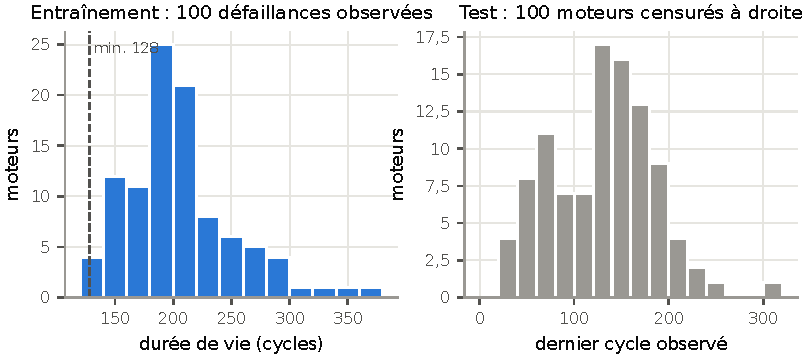
\includegraphics[width=1\linewidth]{figures/donnees_durees_de_vie.pdf}
\caption{Durées de vie des moteurs d'entraînement (gauche) et durées observées, censurées à droite, des moteurs de test (droite).}\label{fig:donnees_durees_de_vie}
\end{figure}

\subsection{Capteurs constants}\label{sec:donnees-capteurs}

Avec une seule condition opératoire, 7 capteurs prennent moins de 10 valeurs distinctes et sont écartés (s1, s5, s6, s10, s16, s18, s19), de même que les réglages opérationnels. Les autres capteurs dérivent progressivement au cours de la vie, avec un bruit important d'un cycle à l'autre, d'où l'usage de moyennes glissantes.

\chapconclusion

Ce chapitre a fixé le cadre et les méthodes de référence de l'étude. Le jeu FD001 fournit 200 unités pour la fiabilité, dont 100 censurées, sans défaillance avant 128 cycles. Le chapitre suivant présente les méthodes appliquées à ces données.

% généré depuis source/05_methodologie.md — ne pas modifier à la main
\chapter{Méthodologie}\label{sec:methodologie}

\chapintro

Ce chapitre présente les méthodes de l'étude : la fiabilité, la maintenabilité et la disponibilité, l'indicateur de santé, la classification de l'état et les deux modèles de RUL. Les valeurs des paramètres sont regroupées au tableau~\ref{tab:hypotheses_parametres} (annexe A).

\section{Fiabilité}\label{sec:fiabilite}

\subsection{Estimation non paramétrique}

Soient $t_1 < t_2 < \dots$ les instants de défaillance, $d_i$ le nombre de défaillances en $t_i$ et $n_i$ le nombre d'unités encore à risque juste avant $t_i$. L'estimateur KM \cite{kaplanmeier1958} est

\begin{equation}\label{eq:km}
\hat R(t) = \prod_{t_i \le t} \left(1 - \frac{d_i}{n_i}\right).
\end{equation}

Une unité censurée sort de l'effectif à risque sans être comptée comme défaillance. L'IC à $95\,\%$ utilise la variance de Greenwood \cite{greenwood1926} sur l'échelle $\log(-\log \hat R)$. La censure est supposée non informative, ce que justifie le tirage indépendant des instants de troncature dans C-MAPSS \cite{saxena2008damage}. Le taux cumulé de Nelson-Aalen, lissé par un noyau d'Epanechnikov de 15 cycles, donne la forme de $\lambda(t)$ sans supposer de loi.

\subsection{Lois paramétriques}

La loi de Weibull à trois paramètres \cite{weibull1951} s'écrit

\begin{equation}\label{eq:weibull3}
R(t) = \exp\!\left[-\left(\frac{t-\gamma}{\eta}\right)^{\beta}\right] \text{ pour } t > \gamma, \qquad R(t) = 1 \text{ sinon},
\end{equation}

avec $\beta$ la forme, $\eta$ l'échelle et $\gamma$ la position, durée sans défaillance garantie ; la loi 2P correspond à $\gamma = 0$. Par \textbf{MCO}, la méthode graphique du cours \cite{benhmida}, les durées triées reçoivent les rangs de Bernard \cite{bernard1953} et la loi 2P se linéarise :

\begin{equation}\label{eq:bernard}
\hat F_i = \frac{i - 0{,}3}{n + 0{,}4}, \qquad \ln\!\big(-\ln(1-\hat F_i)\big) = \beta \ln t_i - \beta \ln \eta .
\end{equation}

Une courbure du diagramme signale un $\gamma$ non nul. Par \textbf{MV}, la log-vraisemblance $\ell = \sum_i [\delta_i \ln f(t_i) + (1-\delta_i) \ln R(t_i)]$ est maximisée. La loi 2P est ajustée avec censure sur les 200 unités (bibliothèque lifelines \cite{davidsonpilon2019}). Les quatre lois candidates, exponentielle, Weibull 2P, log-normale et Weibull 3P, sont comparées sur les 100 durées de défaillance complètes : \textbf{la Weibull 3P retenue est donc ajustée sans les censures}, limite discutée au section~\ref{sec:limites}. L'adéquation est jugée par le test KS au seuil de $5\,\%$, et les lois sont comparées par $\mathrm{AIC} = 2k - 2\ell$ ; un écart inférieur à deux unités les rend équivalentes.

\subsection{Indicateurs dérivés}

Pour la Weibull 3P, le MTTF et la durée $B_p$ valent

\begin{equation}\label{eq:mttf}
\mathrm{MTTF} = \gamma + \eta\, \Gamma\!\left(1 + \frac{1}{\beta}\right), \qquad B_p = \gamma + \eta \big(-\ln(1-p)\big)^{1/\beta}.
\end{equation}

\section{Maintenabilité, disponibilité et remplacement préventif}\label{sec:fmds02}

C-MAPSS ne contient aucun temps de réparation : ils sont donc \textbf{simulés}, selon une loi log-normale de médiane 16 h et d'écart-type logarithmique 0,6, avec un cycle d'environ 2 h. Les résultats qui en dépendent illustrent la démarche du cours et ne décrivent pas une flotte réelle.

La loi log-normale est ré-estimée par MV sur l'échantillon simulé, ce qui donne $\mathrm{MTTR} = e^{\mu + \sigma^2/2}$. La disponibilité intrinsèque d'un moteur réparé après chaque défaillance est

\begin{equation}\label{eq:dispo}
A_\infty = \frac{\mathrm{MUT}}{\mathrm{MUT} + \mathrm{MDT}}, \qquad \mathrm{MUT} = \mathrm{MTTF}, \quad \mathrm{MDT} = \mathrm{MTTR}.
\end{equation}

Selon la politique de Barlow et Proschan \cite{barlow1965}, un moteur est remplacé à l'âge $T$ pour un coût $C_p$, alors qu'une défaillance en service coûte $C_c > C_p$. Le coût moyen par cycle est

\begin{equation}\label{eq:cout}
C(T) = \frac{C_p\, R(T) + C_c\, \big(1 - R(T)\big)}{\displaystyle\int_0^T R(t)\, \mathrm{d}t}, \qquad C_\infty = \frac{C_c}{\mathrm{MTTF}} ,
\end{equation}

où $C_\infty$ est le coût de la maintenance corrective seule. L'âge optimal $T^*$ minimise $C(T)$. Les coûts relatifs $C_p = 1$ et $C_c = 5$ sont une hypothèse d'illustration.

\section{Sélection des capteurs et indicateur de santé}\label{sec:hi}

Pour chaque capteur non constant, deux scores inspirés de Coble et Hines \cite{coble2009} sont calculés : la \textbf{tendance} $\rho$, corrélation moyenne avec le numéro de cycle, et la \textbf{monotonie} de la série lissée,

\begin{equation}\label{eq:monotonie}
\mathrm{Mon} = \frac{|N^{+} - N^{-}|}{n-1},
\end{equation}

où $N^{+}$ et $N^{-}$ sont les nombres de variations positives et négatives et $n$ la longueur de la série. Un capteur est retenu si $|\rho| \ge 0{,}5$. Pour chaque capteur retenu, la moyenne, l'écart-type et la pente sont calculés sur une fenêtre glissante de 10 cycles, moteur par moteur ; avec le HI et le numéro de cycle, chaque cycle est décrit par 38 variables.

Suivant Wang et al. \cite{wang2008}, le HI est une combinaison linéaire des capteurs standardisés $z_j$ :

\begin{equation}\label{eq:hi}
\mathrm{HI}(t) = a_0 + \sum_j a_j\, z_j(t),
\end{equation}

ajustée par moindres carrés vers une cible égale à un sur les 10 \% premiers cycles de chaque moteur et à zéro sur les 10 \% derniers, puis lissée sur 10 cycles.

\section{Classification de l'état de santé}\label{sec:classification}

Un cycle est \textbf{critique} si sa RUL réelle est d'au plus 30 cycles. Deux classifieurs de scikit-learn \cite{pedregosa2011} sont comparés : un gradient boosting à histogrammes \cite{friedman2001,ke2017} et un SVM à noyau gaussien \cite{cortes1995} calibré par la méthode de Platt \cite{platt1999}. Les cycles d'un même moteur étant corrélés, la validation croisée se fait \textbf{par groupes de moteurs} (GroupKFold, 5 plis), sans fuite entre apprentissage et validation. Au dernier cycle observé, chaque moteur est classé \emph{critique} si sa probabilité dépasse $0{,}5$, \emph{surveillance} si elle dépasse 0,2, \emph{normal} sinon.

\section{RUL par modèle de dégradation bayésien}\label{sec:degradation}

Le HI d'un moteur est modélisé par un polynôme de degré 2 du temps réduit $\tau = t/100$, à coefficients propres au moteur :

\begin{equation}\label{eq:degradation}
\mathrm{HI}(t) = \boldsymbol\phi(t)^\top \mathbf w + \varepsilon, \qquad \boldsymbol\phi(t) = (1, \tau, \tau^2)^\top, \qquad \varepsilon \sim \mathcal N(0, \sigma^2).
\end{equation}

Les ajustements sur les moteurs d'entraînement donnent l'a priori de flotte $\mathbf w \sim \mathcal N(\mathbf m_0, \mathbf S_0)$ \cite{gebraeel2005}, la variance $\sigma^2$ des résidus et un seuil de défaillance $\mathcal N(\bar s, \sigma_s^2)$. Pour un moteur observé, de matrice de régression $\boldsymbol\Phi$ et de mesures $\mathbf h$, la loi a posteriori est gaussienne :

\begin{equation}\label{eq:posterior}
\mathbf S_n^{-1} = \mathbf S_0^{-1} + \frac{\boldsymbol\Phi^\top \boldsymbol\Phi}{\sigma^2}, \qquad \mathbf m_n = \mathbf S_n \left(\mathbf S_0^{-1} \mathbf m_0 + \frac{\boldsymbol\Phi^\top \mathbf h}{\sigma^2}\right).
\end{equation}

On tire 1\,000 couples de coefficients et de seuils ; le premier passage de chaque trajectoire sous le seuil donne une RUL. La médiane est la prédiction, et les quantiles donnent les intervalles P25–P75, P10–P90 et P05–P95. Le bruit $\varepsilon$ n'est pas propagé dans les trajectoires.

\section{RUL par réseau LSTM}\label{sec:lstm}

Les 12 capteurs retenus sont normalisés entre zéro et un, et chaque exemple est une fenêtre de 30 cycles d'un même moteur. Suivant Heimes \cite{heimes2008}, la cible est plafonnée, $y = \min(\mathrm{RUL}, 125)$, car la dégradation n'est pas observable en début de vie. Le réseau \cite{hochreiter1997,zheng2017} comprend 2 couches LSTM de 64 unités, une couche dense et une sortie linéaire ; il est entraîné avec Adam \cite{kingma2015} sous PyTorch \cite{paszke2019}, avec un arrêt précoce sur 15 moteurs de validation.

\chapconclusion

Ce chapitre a présenté les méthodes et leurs hypothèses, en particulier la censure non informative et les temps de réparation simulés. Le chapitre suivant les évalue sur les données de test et présente leur restitution.

% généré depuis source/06_evaluation_visualisation.md — ne pas modifier à la main
\chapter{Évaluation et visualisation}\label{sec:evaluation}

\chapintro

Ce chapitre évalue d'abord la solution : protocole et métriques, puis résultats de fiabilité, de disponibilité, de détection de l'état critique et de RUL, et comparaison des méthodes. Il montre ensuite comment ces résultats sont restitués dans le tableau de bord et comment leur reproductibilité est assurée.

\section{Protocole et métriques}\label{sec:protocole}

Le découpage officiel de FD001 est respecté : les modèles sont appris sur les 100 moteurs d'entraînement et évalués sur les 100 moteurs de test. La fiabilité porte sur les 200 unités avec censure ; la classification est validée par GroupKFold puis évaluée sur tous les cycles de test ; la RUL est évaluée au dernier cycle observé de chaque moteur, comme dans le challenge PHM \cite{saxena2008damage}.

Pour la classification, la classe positive est l'état critique. Le \textbf{rappel} est la métrique prioritaire, car une défaillance manquée coûte bien plus qu'une inspection inutile ; l'AUC \cite{hanley1982} mesure la qualité du classement indépendamment du seuil. Pour la RUL, l'erreur d'un moteur est $e_i = \widehat{\mathrm{RUL}}_i - \mathrm{RUL}_i$ ; une erreur positive est une prédiction \textbf{tardive}, la plus dangereuse. Sur $N$ moteurs :

\begin{equation}\label{eq:rmse}
\mathrm{RMSE} = \sqrt{\frac1N \sum_i e_i^2}, \qquad \mathrm{MAE} = \frac1N \sum_i |e_i|, \qquad S = \sum_i \begin{cases} e^{-e_i/13} - 1 & e_i < 0 \\ e^{e_i/10} - 1 & e_i \ge 0 \end{cases},
\end{equation}

où $S$ est le score NASA \cite{saxena2008damage}. La \textbf{couverture} d'un intervalle de prédiction est la proportion de moteurs dont la RUL réelle y tombe ; elle doit être proche du niveau nominal.

\section{Fiabilité}\label{sec:res-fiabilite}

La figure~\ref{fig:fiabilite_kaplan_meier} compare l'estimateur KM aux lois ajustées ; la médiane de survie vaut 202 cycles. Les censures, concentrées aux faibles âges, élargissent peu l'IC. Le taux de Nelson-Aalen, nul avant la première défaillance puis croissant, confirme une \textbf{usure}.

\begin{figure}[htbp]
\centering
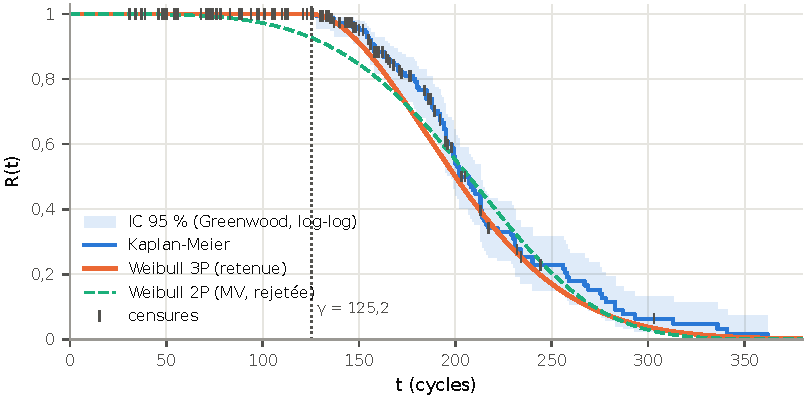
\includegraphics[width=1\linewidth]{figures/fiabilite_kaplan_meier.pdf}
\caption{Fonction de fiabilité : estimateur KM avec son IC et les censures, loi de Weibull 3P retenue et loi de Weibull 2P (MV) rejetée.}\label{fig:fiabilite_kaplan_meier}
\end{figure}

Le diagramme de Weibull (figure~\ref{fig:fiabilite_diagramme_weibull}) est nettement courbé ($R^2 = 0{,}894$, $\beta = 5{,}52$ par MCO), ce qui révèle un paramètre de position non nul.

\begin{figure}[htbp]
\centering
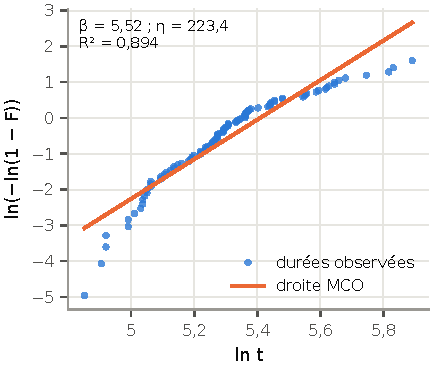
\includegraphics[width=0.55\linewidth]{figures/fiabilite_diagramme_weibull.pdf}
\caption{Diagramme de Weibull (rangs de Bernard) et droite des MCO : la courbure révèle un paramètre de position non nul.}\label{fig:fiabilite_diagramme_weibull}
\end{figure}

Le tableau~\ref{tab:fiabilite_adequation} compare les quatre lois candidates.

\begin{table}[htbp]
\centering\small
\begin{adjustbox}{max width=\linewidth,center}
\begin{tabular}{lrrrrrl}
\toprule
Loi & Paramètres & Log-vraisemblance & AIC & KS D & KS p & Décision (\ensuremath{\alpha} = 5 \%) \\
\midrule
Exponentielle & 1 & \ensuremath{-}632,94 & 1\,267,88 & 0,470 & 0,000 & rejetée \\
Weibull 2P & 2 & \ensuremath{-}530,75 & 1\,065,50 & 0,157 & 0,013 & rejetée \\
Log-normale & 2 & \ensuremath{-}517,46 & 1\,038,91 & 0,094 & 0,317 & acceptée \\
Weibull 3P & 3 & \ensuremath{-}516,52 & 1\,039,03 & 0,094 & 0,319 & acceptée \\
\bottomrule
\end{tabular}
\end{adjustbox}
\caption{Adéquation des lois candidates (MV sur les durées complètes)}\label{tab:fiabilite_adequation}
\end{table}

La loi exponentielle et la Weibull 2P (MV, $\beta = 4{,}41$, $p = 0{,}013$) sont rejetées. La Weibull 3P et la log-normale sont acceptées et équivalentes ($\Delta\mathrm{AIC} = 0{,}12$). La \textbf{Weibull 3P est retenue} : $\gamma = 125{,}2$ cycles traduit une période sans défaillance cohérente avec la première défaillance à 128 cycles, $\beta = 1{,}83 > 1$ un taux croissant, et c'est la loi de référence du cours \cite{benhmida}. L'ajustement 2P avec censure donne une échelle plus grande ($\eta = 236{,}6$ cycles), car les moteurs censurés ont survécu au moins jusqu'à leur dernier cycle. Le tableau~\ref{tab:fiabilite_indicateurs} donne les indicateurs du modèle retenu.

\begin{table}[htbp]
\centering\small
\begin{adjustbox}{max width=\linewidth,center}
\begin{tabular}{lrl}
\toprule
Indicateur & Valeur & Source \\
\midrule
MTTF = \ensuremath{\gamma} + \ensuremath{\eta}·\ensuremath{\Gamma}(1 + 1/\ensuremath{\beta}) & 206,3 cycles & Weibull 3P \\
B1 (1 \% de défaillances) & 132,6 cycles & Weibull 3P \\
B10 (10 \%) & 151,9 cycles & Weibull 3P \\
B50 (médiane) & 199,9 cycles & Weibull 3P \\
Médiane de survie & 202 cycles & Kaplan-Meier \\
Aire sous la courbe de survie & 214,3 cycles & Kaplan-Meier \\
Première défaillance observée & 128 cycles & données \\
\bottomrule
\end{tabular}
\end{adjustbox}
\caption{Indicateurs de fiabilité}\label{tab:fiabilite_indicateurs}
\end{table}

$B_{50}$ est proche de la médiane KM, ce qui confirme l'accord des deux approches au centre de la distribution. La figure~\ref{fig:fiabilite_densite_repartition} situe $B_{10}$ et $B_{50}$ sur la densité et la fonction de répartition.

\begin{figure}[htbp]
\centering
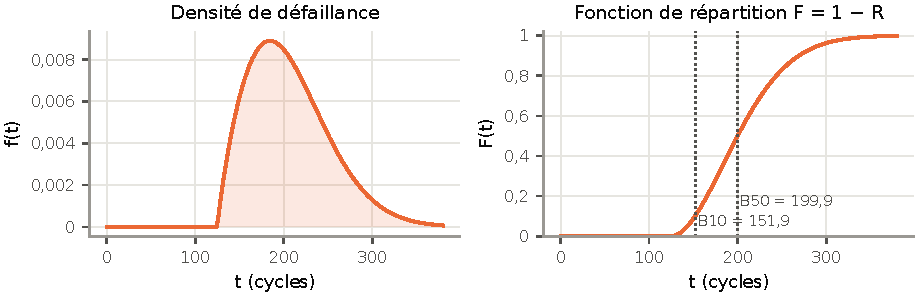
\includegraphics[width=1\linewidth]{figures/fiabilite_densite_repartition.pdf}
\caption{Densité de défaillance et fonction de répartition de la loi de Weibull 3P, avec les durées B10 et B50.}\label{fig:fiabilite_densite_repartition}
\end{figure}

\section{Disponibilité et remplacement préventif}\label{sec:res-fmds02}

Le tableau~\ref{tab:fmds_maintenabilite_disponibilite} regroupe les indicateurs obtenus avec les temps de réparation simulés.

\begin{table}[htbp]
\centering\small
\begin{adjustbox}{max width=\linewidth,center}
\begin{tabular}{ll}
\toprule
Grandeur & Valeur \\
\midrule
Loi des temps de réparation (MV) & log-normale, \ensuremath{\mu} = 2,742, \ensuremath{\sigma} = 0,464 (KS p = 0,61) \\
MTTR & 17,3 h = 8,6 cycles \\
t90 (90 \% des réparations terminées) & 28,1 h \\
MUT / MDT / MTBF & 206,3 / 8,64 / 215,0 cycles \\
Disponibilité intrinsèque A = MUT / (MUT + MDT) & 95,98 \% \\
Âge optimal de remplacement T* & 130,7 cycles, R(T*) = 0,994 \\
Coût par cycle : à T* / corrective seule & 0,0078 / 0,0242 (unités de Cp) \\
Gain du préventif & 67,7 \% \\
\bottomrule
\end{tabular}
\end{adjustbox}
\caption{Maintenabilité, disponibilité et remplacement préventif (temps de réparation simulés)}\label{tab:fmds_maintenabilite_disponibilite}
\end{table}

La loi log-normale ré-estimée est acceptée par le test KS ($p = 0{,}61$). La disponibilité intrinsèque atteint \textbf{95,98 \%}, soit environ 40,2 h d'indisponibilité pour mille heures. La figure~\ref{fig:fmds_remplacement_preventif} montre le coût du remplacement préventif en fonction de l'âge.

\begin{figure}[htbp]
\centering
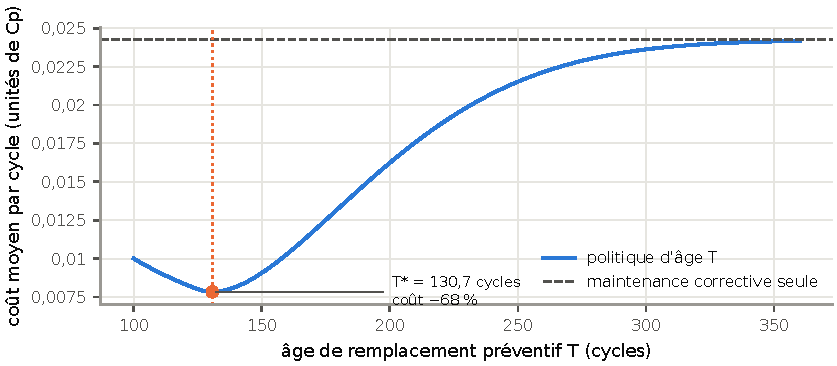
\includegraphics[width=1\linewidth]{figures/fmds_remplacement_preventif.pdf}
\caption{Coût moyen par cycle du remplacement à âge fixe en fonction de l'âge T, comparé à la maintenance corrective seule.}\label{fig:fmds_remplacement_preventif}
\end{figure}

L'optimum, net, se situe à $T^* = 130{,}7$ cycles, juste après la période sans défaillance : le coût par cycle baisse de \textbf{68 \%}, au prix d'un remplacement en moyenne 75,6 cycles avant le MTTF.

\section{Détection de l'état critique}\label{sec:res-sante}

Parmi les capteurs non constants, 12 dépassent le seuil de tendance et sont retenus : s2, s3, s4, s7, s8, s11, s12, s13, s15, s17, s20, s21. La figure~\ref{fig:sante_indicateur} montre le HI obtenu.

\begin{figure}[htbp]
\centering
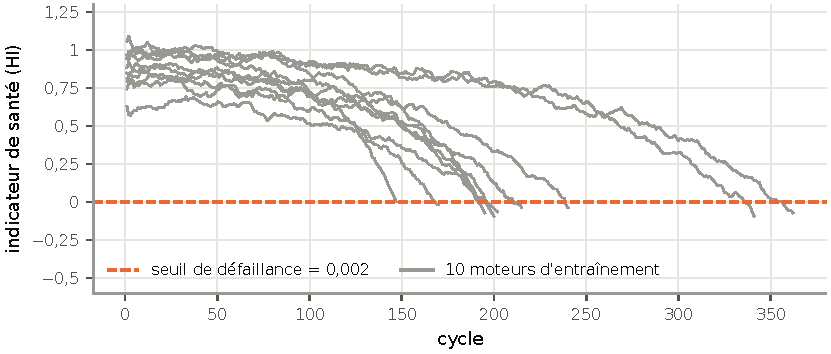
\includegraphics[width=1\linewidth]{figures/sante_indicateur.pdf}
\caption{HI lissé de dix moteurs d'entraînement et seuil de défaillance.}\label{fig:sante_indicateur}
\end{figure}

Le HI part d'environ un et décroît jusqu'au voisinage de zéro pour tous les moteurs, quelle que soit leur durée de vie. Le tableau~\ref{tab:sante_classifieurs} compare les deux classifieurs.

\begin{table}[htbp]
\centering\small
\begin{adjustbox}{max width=\linewidth,center}
\begin{tabular}{llrrrrr}
\toprule
Modèle & Évaluation & AUC & Exactitude & Précision & Rappel & F1 \\
\midrule
Gradient Boosting & validation croisée (GroupKFold 5) & 0,990 & 0,961 & 0,892 & 0,844 & 0,867 \\
 & test NASA & 0,991 & 0,986 & 0,747 & 0,657 & 0,699 \\
SVM (RBF) & validation croisée (GroupKFold 5) & 0,983 & 0,958 & 0,879 & 0,824 & 0,851 \\
 & test NASA & 0,974 & 0,986 & 0,798 & 0,621 & 0,698 \\
\bottomrule
\end{tabular}
\end{adjustbox}
\caption{Classification normal / critique (RUL \ensuremath{\le} 30 cycles)}\label{tab:sante_classifieurs}
\end{table}

Les deux modèles séparent très bien les classes ; le \textbf{gradient boosting}, de meilleure AUC sur le test (0,991), est retenu. Son rappel de test (0,657) est pourtant inférieur à celui de la validation croisée (0,844), comme le détaille la figure~\ref{fig:sante_matrice_confusion}.

\begin{figure}[htbp]
\centering
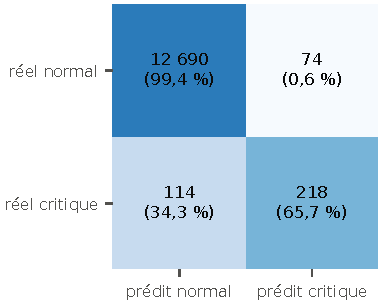
\includegraphics[width=0.50\linewidth]{figures/sante_matrice_confusion.pdf}
\caption{Matrice de confusion du gradient boosting sur le jeu de test, au seuil de décision par défaut.}\label{fig:sante_matrice_confusion}
\end{figure}

Le jeu de test est très déséquilibré : la plupart des séries s'arrêtent bien avant la défaillance. L'AUC reste élevée, c'est donc le seuil de décision qui est trop strict. Au dernier cycle, la flotte compte 76 moteurs normaux, 4 en surveillance et 20 critiques.

\section{Durée de vie résiduelle}\label{sec:res-rul}

Le tableau~\ref{tab:rul_metriques} compare les deux modèles sur les 100 moteurs de test.

\begin{table}[htbp]
\centering\small
\begin{adjustbox}{max width=\linewidth,center}
\begin{tabular}{lrrrrrr}
\toprule
Modèle & RMSE & MAE & Biais & Score NASA & |e| \ensuremath{\le} 15 & Tardives \\
\midrule
Dégradation bayésienne & 24,47 & 18,98 & +13,5 & 3\,743 & 49 \% & 78 \% \\
LSTM & 15,35 & 11,22 & +2,2 & 485 & 68 \% & 58 \% \\
Moyenne des deux & 16,91 & 13,49 & +7,9 & 600 & 64 \% & 76 \% \\
\bottomrule
\end{tabular}
\end{adjustbox}
\caption{Performances des modèles de RUL sur les 100 moteurs de test}\label{tab:rul_metriques}
\end{table}

Le \textbf{LSTM est le plus précis} sur toutes les métriques et presque sans biais. Le modèle de dégradation prédit en moyenne trop tard (+13,5 cycles), ce que le score NASA amplifie. La moyenne des deux n'améliore pas le LSTM seul. La figure~\ref{fig:rul_predit_vs_reel} montre les prédictions en fonction de la RUL réelle.

\begin{figure}[htbp]
\centering
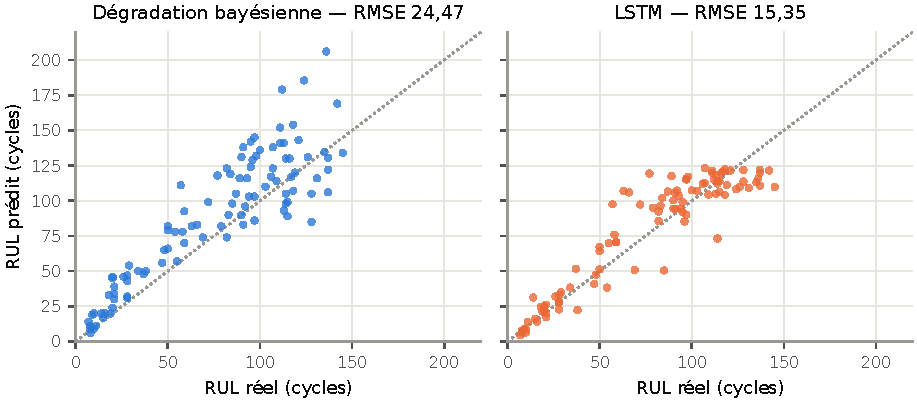
\includegraphics[width=1\linewidth]{figures/rul_predit_vs_reel.pdf}
\caption{RUL prédite en fonction de la RUL réelle pour les deux modèles ; la diagonale correspond à une prédiction parfaite.}\label{fig:rul_predit_vs_reel}
\end{figure}

Le LSTM suit la diagonale jusqu'à son plafond de 125 cycles ; le modèle de dégradation est plus dispersé et majoritairement au-dessus. La figure~\ref{fig:rul_calibration} évalue ses intervalles de prédiction.

\begin{figure}[htbp]
\centering
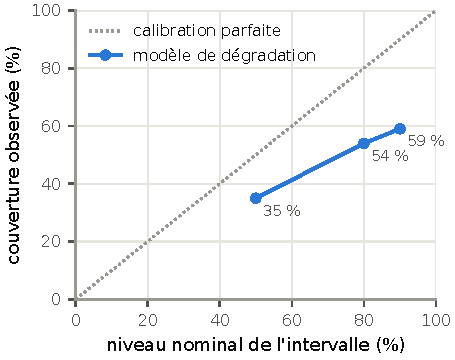
\includegraphics[width=0.55\linewidth]{figures/rul_calibration.pdf}
\caption{Calibration des intervalles du modèle de dégradation : couverture observée en fonction du niveau nominal.}\label{fig:rul_calibration}
\end{figure}

Les couvertures observées, 35 \%, 54 \% et 59 \% pour des niveaux nominaux de 50, 80 et 90 \%, sont toutes trop faibles : \textbf{les intervalles sont trop étroits} et le modèle sous-estime son incertitude. La figure~\ref{fig:rul_exemple_moteur} illustre les deux modèles sur le moteur de test n° 31.

\begin{figure}[htbp]
\centering
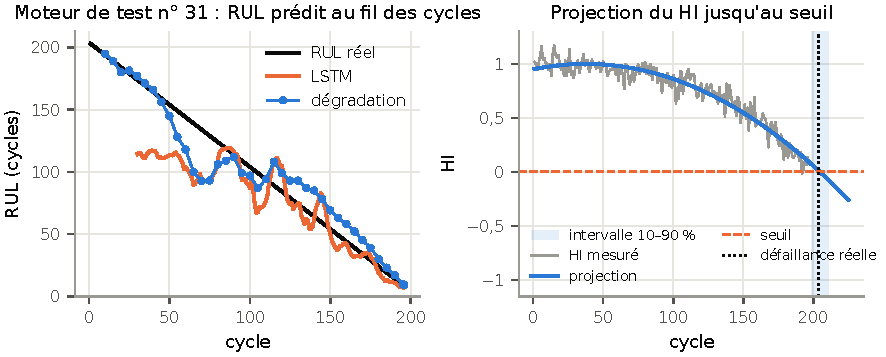
\includegraphics[width=1\linewidth]{figures/rul_exemple_moteur.pdf}
\caption{Moteur de test pris en exemple : RUL prédite à chaque cycle par les deux modèles (gauche) et projection du HI jusqu'au seuil de défaillance (droite).}\label{fig:rul_exemple_moteur}
\end{figure}

Au fil des cycles, les deux prédictions se rapprochent de la RUL réelle (8 cycles) ; la projection du HI montre comment le modèle bayésien déduit la RUL du franchissement du seuil.

\section{Comparaison des méthodes}\label{sec:comparaison}

Les deux approches de RUL sont complémentaires. Le \textbf{LSTM} est précis et quasi sans biais, du même ordre que les réseaux récurrents publiés sur FD001 \cite{zheng2017,ramasso2014}, mais il ne fournit pas d'incertitude et reste peu interprétable. Le \textbf{modèle de dégradation} est moins précis et biaisé, mais chaque étape est interprétable et il fournit une distribution de la RUL, encore mal calibrée. En fiabilité, les approches non paramétrique et paramétrique concordent sur la forme du taux et sur la médiane.

\section{Visualisation : le tableau de bord}\label{sec:dashboard}

Les résultats évalués sont restitués dans un tableau de bord web React, alimenté par une API qui sert les fichiers de résultats ; une version autonome en un seul fichier HTML s'ouvre sans serveur. La page de vue d'ensemble (figure~\ref{fig:dashboard_overview}) réunit les indicateurs clés et l'état de la flotte.

\begin{figure}[htbp]
\centering
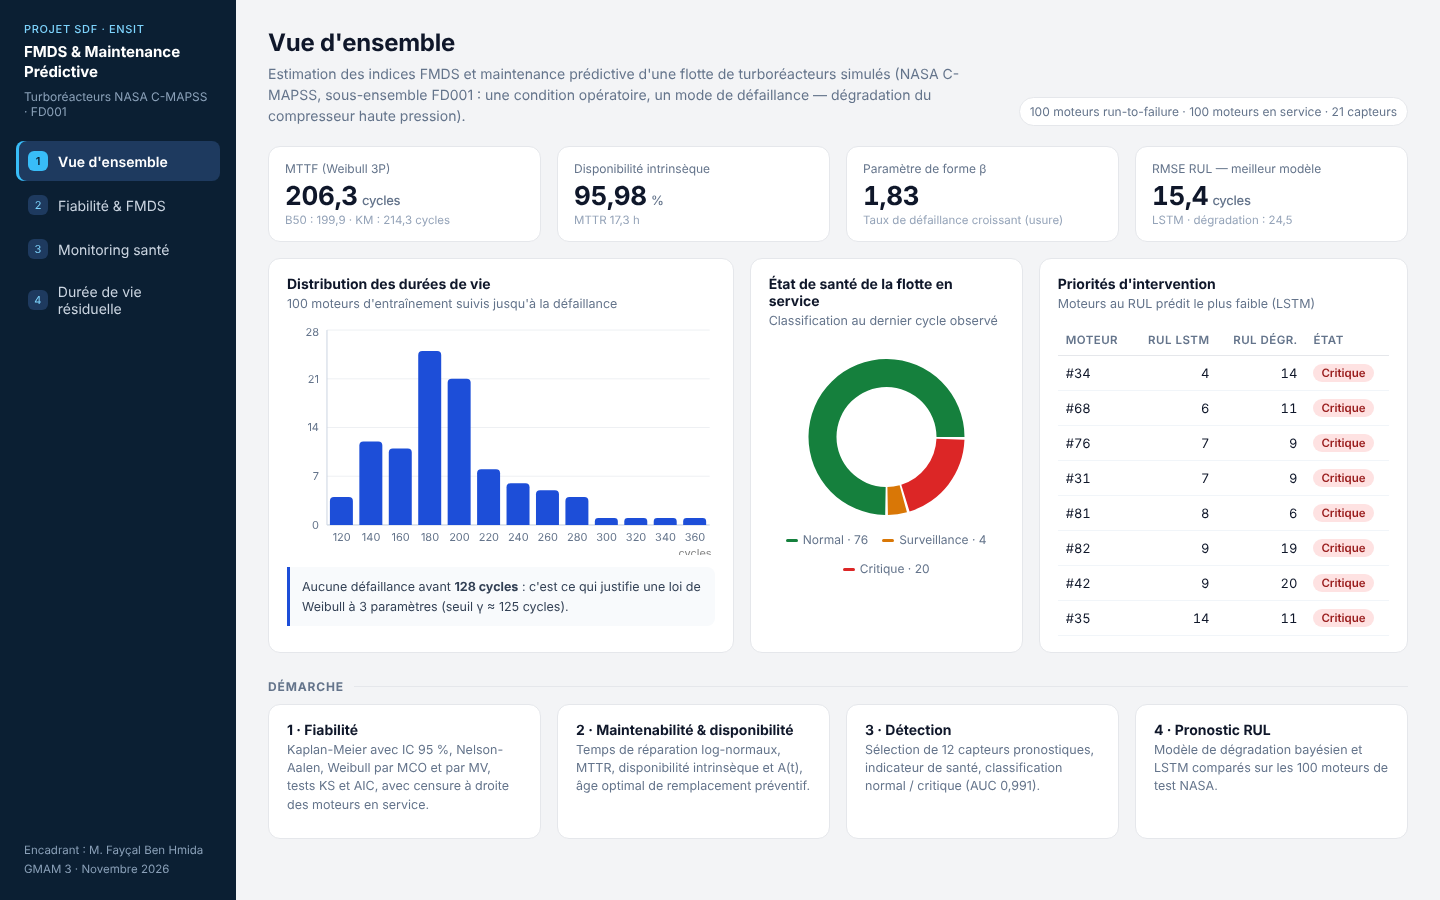
\includegraphics[width=1\linewidth]{figures/dashboard_overview.png}
\caption{Page de vue d'ensemble : indicateurs clés, distribution des durées de vie, état de la flotte et priorités d'intervention.}\label{fig:dashboard_overview}
\end{figure}

La page consacrée à la RUL (figure~\ref{fig:dashboard_rul}) compare les deux modèles et détaille les prédictions pour chaque moteur.

\begin{figure}[htbp]
\centering
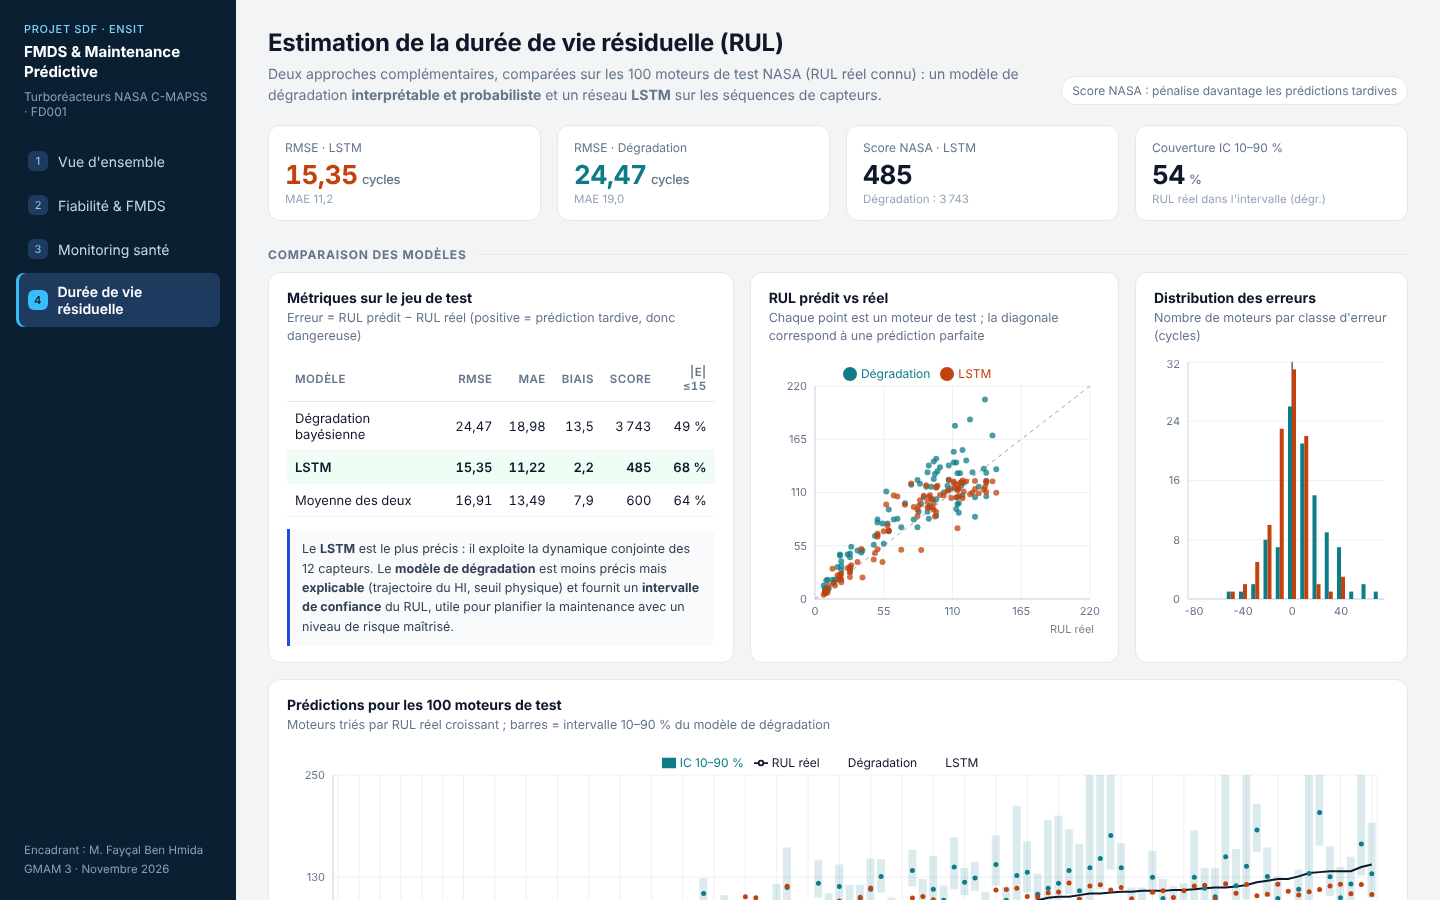
\includegraphics[width=1\linewidth]{figures/dashboard_rul.png}
\caption{Page de la durée de vie résiduelle : métriques des deux modèles, prédictions et erreurs.}\label{fig:dashboard_rul}
\end{figure}

\section{Reproductibilité}\label{sec:reproductibilite}

Toutes les étapes aléatoires utilisent des graines fixées, et chaque exécution enregistre les versions des bibliothèques (Python 3.12.10, scikit-learn 1.9.1, PyTorch 2.15.0). Le réentraînement du LSTM variant légèrement d'une machine à l'autre, les résultats publiés correspondent au modèle sauvegardé. Une suite de tests automatiques vérifie les méthodes, l'absence de fuite entre moteurs et la concordance de chaque nombre du rapport avec sa source.

\chapconclusion

La Weibull 3P décrit la fiabilité de la flotte avec un MTTF de 206,3 cycles, le classifieur atteint une AUC de 0,991, et le LSTM est le plus précis pour la RUL (RMSE de 15,35 cycles), tandis que le modèle de dégradation fournit des intervalles encore trop étroits. Le chapitre suivant discute ces résultats.

% généré depuis source/07_discussion_perspectives.md — ne pas modifier à la main
\chapter{Discussion et perspectives}\label{sec:discussion}

\chapintro

Ce chapitre interprète les résultats dans le contexte industriel, en présente les limites, puis propose les travaux futurs prioritaires.

\section{Interprétation industrielle}\label{sec:interpretation}

\textbf{Une flotte qui s'use.} Le paramètre de forme supérieur à un et le taux croissant signent des défaillances d'usure, conformes à la dégradation simulée du HPC : remplacer un moteur âgé réduit réellement le risque.

\textbf{Une période sans défaillance.} Le paramètre $\gamma$ permet d'alléger les inspections en début de vie et de concentrer la surveillance au-delà de cet âge.

\textbf{Le préventif et ses limites.} Le remplacement à $T^*$ réduit fortement le coût par cycle sous l'hypothèse de coûts retenue, mais il remplace aussi les moteurs robustes et sacrifie en moyenne 75,6 cycles de vie utile.

\textbf{L'apport du prédictif.} Le HI, la détection de l'état critique et la RUL permettent de décider moteur par moteur : le classifieur peut servir d'alarme et le modèle de RUL de planification, le LSTM apportant la précision et le modèle bayésien l'explication et l'incertitude.

\section{Limites}\label{sec:limites}

\begin{itemize}
\item \textbf{Hypothèses simulées.} Les temps de réparation, la conversion d'un cycle en 2 h et le rapport de coûts sont supposés : la maintenabilité, la disponibilité et le coût illustrent la démarche, sans valeur industrielle.
\item \textbf{Un seul sous-ensemble.} FD001 n'a qu'une condition opératoire et un mode de défaillance ; les conclusions ne s'étendent pas telles quelles à FD002–FD004.
\item \textbf{Weibull 3P ajustée sans censure.} L'aire sous la courbe KM (214,3 cycles) dépasse le MTTF du modèle (206,3 cycles) : le modèle sous-estime probablement un peu les durées de vie.
\item \textbf{Biais et sous-couverture du modèle de dégradation.} La base polynomiale extrapole mal une dégradation qui s'accélère, le bruit n'est pas propagé et le seuil est estimé sur des valeurs ajustées ; ce modèle ne doit pas décider seul.
\item \textbf{Seuil du classifieur.} Le rappel de test est faible au seuil par défaut ; ce seuil devrait refléter le coût relatif d'une défaillance manquée et d'une fausse alerte.
\item \textbf{Évaluation ponctuelle de la RUL.} Seul le dernier cycle de chaque moteur de test est évalué ; le suivi au fil de la vie n'est illustré que sur un exemple.
\end{itemize}

\section{Travaux futurs}\label{sec:travaux-futurs}

Cinq travaux futurs sont prioritaires ; aucun n'est réalisé à ce stade.

\begin{itemize}
\item \textbf{Modèle de dégradation exponentiel ou de Wiener.} Remplacer la base polynomiale par un modèle exponentiel à coefficients aléatoires ou un processus de Wiener à dérive non linéaire \cite{gebraeel2005,si2012} devrait réduire le biais tardif, en comparant RMSE, biais et score NASA sur les mêmes moteurs.
\item \textbf{Intervalles calibrés.} Propager le bruit de mesure dans les trajectoires puis recalibrer les intervalles sur des moteurs réservés, par exemple par prédiction conforme, viserait une couverture proche du niveau nominal.
\item \textbf{Weibull 3P avec censure et incertitude des $B_p$.} Ajuster la loi retenue par MV avec censure et donner des IC de $B_{10}$ et $B_{50}$ par bootstrap \cite{efron1979} lèverait la limite principale de l'analyse de fiabilité.
\item \textbf{Conditions opératoires multiples.} Étendre l'étude à FD002 et FD004, avec une normalisation par condition et un modèle de Cox \cite{cox1972}, rendrait les modèles transposables à des usages variés.
\item \textbf{Données et coûts réels.} Remplacer les hypothèses simulées par des temps de réparation et des coûts réels permettrait une véritable étude économique du préventif et du prédictif.
\end{itemize}

\chapconclusion

Les résultats confirment l'intérêt de combiner une vision de flotte, par les indices FMDS, et une décision moteur par moteur, par le pronostic. Les limites identifiées, surtout la calibration du modèle de dégradation et le caractère simulé de certaines hypothèses, fixent les travaux futurs.

% généré depuis source/08_conclusion_generale.md — ne pas modifier à la main
\chapter*{Conclusion générale}
\addcontentsline{toc}{chapter}{Conclusion générale}
\frontmark{Conclusion générale}

Ce projet a appliqué l'ensemble de la démarche de sûreté de fonctionnement à une flotte de turboréacteurs simulés, des données brutes jusqu'à un outil d'aide à la décision.

L'analyse de fiabilité, menée en tenant compte des 100 moteurs censurés, montre une flotte soumise à l'usure, avec une période sans défaillance. La loi de Weibull à trois paramètres, acceptée par le test KS et équivalente à la log-normale selon l'AIC, donne un MTTF de 206,3 cycles et des durées $B_{10}$ et $B_{50}$ de 151,9 et 199,9 cycles. Sous des hypothèses de réparation et de coût explicitement signalées, la disponibilité intrinsèque atteint 95,98 \% et un remplacement préventif à 131 cycles réduit le coût par cycle de 68 \%.

La chaîne de maintenance prédictive complète cette vision par une décision moteur par moteur. Un HI construit sur 12 capteurs décrit la dégradation, le classifieur détecte l'état critique avec une AUC de 0,991, et deux modèles estiment la RUL. Le LSTM est le plus précis (RMSE de 15,35 cycles) ; le modèle de dégradation bayésien, moins précis (RMSE de 24,47 cycles), est interprétable et probabiliste, et son biais comme la calibration insuffisante de ses intervalles sont mesurés et expliqués.

Les résultats sont restitués dans un tableau de bord et produits par un système reproductible. Les travaux futurs prioritaires portent sur un modèle de dégradation plus fidèle et mieux calibré, l'ajustement de la loi retenue avec censure et l'extension à plusieurs conditions opératoires.

% généré depuis source/09_bibliographie.md — ne pas modifier à la main

\chapter*{Bibliographie}
\addcontentsline{toc}{chapter}{Bibliographie}
\frontmark{Bibliographie}
\begin{multicols}{2}
\small\setstretch{1.15}\sloppy
\begingroup
\renewcommand{\chapter}[2]{}% le titre est déjà imprimé
\begin{thebibliography}{99}
\setlength{\itemsep}{2pt}
\bibitem{saxena2008data} A. Saxena and K. Goebel, ``Turbofan engine degradation simulation data set,'' NASA Ames Prognostics Data Repository, NASA Ames Research Center, Moffett Field, CA, 2008.
\bibitem{saxena2008damage} A. Saxena, K. Goebel, D. Simon, and N. Eklund, ``Damage propagation modeling for aircraft engine run-to-failure simulation,'' in \emph{Proc. Int. Conf. Prognostics and Health Management (PHM)}, 2008.
\bibitem{nf13306} AFNOR, \emph{Maintenance — Terminologie de la maintenance}, NF EN 13306, 2018.
\bibitem{jardine2006} A. K. S. Jardine, D. Lin, and D. Banjevic, ``A review on machinery diagnostics and prognostics implementing condition-based maintenance,'' \emph{Mech. Syst. Signal Process.}, vol. 20, no. 7, pp. 1483–1510, 2006.
\bibitem{benhmida} F. Ben Hmida, ``Estimation des indices FMDS,'' Support de cours, module « Sûreté de fonctionnement et maintenance », GMAM 3, ENSIT, Tunis, 2025.
\bibitem{lei2018} Y. Lei, N. Li, L. Guo, N. Li, T. Yan, and J. Lin, ``Machinery health prognostics: A systematic review from data acquisition to RUL prediction,'' \emph{Mech. Syst. Signal Process.}, vol. 104, pp. 799–834, 2018.
\bibitem{si2011} X.-S. Si, W. Wang, C.-H. Hu, and D.-H. Zhou, ``Remaining useful life estimation — A review on the statistical data driven approaches,'' \emph{Eur. J. Oper. Res.}, vol. 213, no. 1, pp. 1–14, 2011.
\bibitem{kaplanmeier1958} E. L. Kaplan and P. Meier, ``Nonparametric estimation from incomplete observations,'' \emph{J. Amer. Statist. Assoc.}, vol. 53, no. 282, pp. 457–481, 1958.
\bibitem{greenwood1926} M. Greenwood, ``The natural duration of cancer,'' His Majesty's Stationery Office, London, Reports on Public Health and Medical Subjects 33, 1926.
\bibitem{nelson1972} W. Nelson, ``Theory and applications of hazard plotting for censored failure data,'' \emph{Technometrics}, vol. 14, no. 4, pp. 945–966, 1972.
\bibitem{aalen1978} O. Aalen, ``Nonparametric inference for a family of counting processes,'' \emph{Ann. Statist.}, vol. 6, no. 4, pp. 701–726, 1978.
\bibitem{weibull1951} W. Weibull, ``A statistical distribution function of wide applicability,'' \emph{J. Appl. Mech.}, vol. 18, pp. 293–297, 1951.
\bibitem{bernard1953} A. Bernard and E. C. Bos-Levenbach, ``The plotting of observations on probability paper,'' \emph{Statistica Neerlandica}, vol. 7, pp. 163–173, 1953.
\bibitem{massey1951} F. J. Massey, ``The Kolmogorov-Smirnov test for goodness of fit,'' \emph{J. Amer. Statist. Assoc.}, vol. 46, no. 253, pp. 68–78, 1951.
\bibitem{akaike1974} H. Akaike, ``A new look at the statistical model identification,'' \emph{IEEE Trans. Autom. Control}, vol. 19, no. 6, pp. 716–723, 1974.
\bibitem{barlow1965} R. E. Barlow and F. Proschan, \emph{Mathematical Theory of Reliability}. New York, NY, USA: Wiley, 1965.
\bibitem{coble2009} J. Coble and J. W. Hines, ``Identifying optimal prognostic parameters from data: A genetic algorithms approach,'' in \emph{Proc. Annu. Conf. Prognostics and Health Management Society}, 2009.
\bibitem{wang2008} T. Wang, J. Yu, D. Siegel, and J. Lee, ``A similarity-based prognostics approach for remaining useful life estimation of engineered systems,'' in \emph{Proc. Int. Conf. Prognostics and Health Management (PHM)}, 2008.
\bibitem{gebraeel2005} N. Z. Gebraeel, M. A. Lawley, R. Li, and J. K. Ryan, ``Residual-life distributions from component degradation signals: A Bayesian approach,'' \emph{IIE Trans.}, vol. 37, no. 6, pp. 543–557, 2005.
\bibitem{si2012} X.-S. Si, W. Wang, C.-H. Hu, D.-H. Zhou, and M. G. Pecht, ``Remaining useful life estimation based on a nonlinear diffusion degradation process,'' \emph{IEEE Trans. Rel.}, vol. 61, no. 1, pp. 50–67, 2012.
\bibitem{heimes2008} F. O. Heimes, ``Recurrent neural networks for remaining useful life estimation,'' in \emph{Proc. Int. Conf. Prognostics and Health Management (PHM)}, 2008.
\bibitem{hochreiter1997} S. Hochreiter and J. Schmidhuber, ``Long short-term memory,'' \emph{Neural Comput.}, vol. 9, no. 8, pp. 1735–1780, 1997.
\bibitem{zheng2017} S. Zheng, K. Ristovski, A. Farahat, and C. Gupta, ``Long short-term memory network for remaining useful life estimation,'' in \emph{Proc. IEEE Int. Conf. Prognostics and Health Management (ICPHM)}, 2017.
\bibitem{babu2016} G. S. Babu, P. Zhao, and X.-L. Li, ``Deep convolutional neural network based regression approach for estimation of remaining useful life,'' in \emph{Database Systems for Advanced Applications (DASFAA)}, ser. Lecture Notes in Computer Science, vol. 9642. Springer, 2016.
\bibitem{li2018} X. Li, Q. Ding, and J.-Q. Sun, ``Remaining useful life estimation in prognostics using deep convolution neural networks,'' \emph{Reliab. Eng. Syst. Saf.}, vol. 172, pp. 1–11, 2018.
\bibitem{ramasso2014} E. Ramasso and A. Saxena, ``Performance benchmarking and analysis of prognostic methods for CMAPSS datasets,'' \emph{Int. J. Prognostics and Health Management}, vol. 5, no. 2, 2014.
\bibitem{davidsonpilon2019} C. Davidson-Pilon, ``lifelines: Survival analysis in Python,'' \emph{J. Open Source Softw.}, vol. 4, no. 40, pp. 1317, 2019.
\bibitem{pedregosa2011} F. Pedregosa et al., ``Scikit-learn: Machine learning in Python,'' \emph{J. Mach. Learn. Res.}, vol. 12, pp. 2825–2830, 2011.
\bibitem{friedman2001} J. H. Friedman, ``Greedy function approximation: A gradient boosting machine,'' \emph{Ann. Statist.}, vol. 29, no. 5, pp. 1189–1232, 2001.
\bibitem{ke2017} G. Ke, Q. Meng, T. Finley, T. Wang, W. Chen, W. Ma, Q. Ye, and T.-Y. Liu, ``LightGBM: A highly efficient gradient boosting decision tree,'' in \emph{Advances in Neural Information Processing Systems (NeurIPS)}, vol. 30, 2017.
\bibitem{cortes1995} C. Cortes and V. Vapnik, ``Support-vector networks,'' \emph{Mach. Learn.}, vol. 20, pp. 273–297, 1995.
\bibitem{platt1999} J. Platt, ``Probabilistic outputs for support vector machines and comparisons to regularized likelihood methods,'' in \emph{Advances in Large Margin Classifiers}. Cambridge, MA, USA: MIT Press, 1999.
\bibitem{kingma2015} D. P. Kingma and J. Ba, ``Adam: A method for stochastic optimization,'' in \emph{Proc. Int. Conf. Learning Representations (ICLR)}, 2015.
\bibitem{paszke2019} A. Paszke et al., ``PyTorch: An imperative style, high-performance deep learning library,'' in \emph{Advances in Neural Information Processing Systems (NeurIPS)}, vol. 32, 2019.
\bibitem{hanley1982} J. A. Hanley and B. J. McNeil, ``The meaning and use of the area under a receiver operating characteristic (ROC) curve,'' \emph{Radiology}, vol. 143, no. 1, pp. 29–36, 1982.
\bibitem{efron1979} B. Efron, ``Bootstrap methods: Another look at the jackknife,'' \emph{Ann. Statist.}, vol. 7, no. 1, pp. 1–26, 1979.
\bibitem{cox1972} D. R. Cox, ``Regression models and life-tables,'' \emph{J. Roy. Statist. Soc. B}, vol. 34, no. 2, pp. 187–220, 1972.
\end{thebibliography}
\endgroup
\end{multicols}

% généré depuis source/10_annexes.md — ne pas modifier à la main
\chapter*{Annexes}
\addcontentsline{toc}{chapter}{Annexes}
\frontmark{Annexes}

\section*{Annexe A — Hypothèses et paramètres}

\begin{table}[htbp]
\centering\small
\begin{adjustbox}{max width=\linewidth,center}
\begin{tabular}{lll}
\toprule
Paramètre & Valeur & Module \\
\midrule
Conversion temps & 1 cycle \ensuremath{\approx} 2 h (1 vol) & fmds.py \\
Temps de réparation simulés & log-normale, médiane 16 h, \ensuremath{\sigma} = 0,6, graine 42 & fmds.py \\
Coûts relatifs & Cp = 1, Cc = 5 & fmds.py \\
Capteur constant & moins de 10 valeurs distinctes & features.py \\
Sélection des capteurs & |tendance| \ensuremath{\ge} 0,5 & features.py \\
Fenêtre glissante (features, lissage du HI) & 10 cycles & features.py \\
Cible du HI & 1 sur les 10 \% premiers cycles, 0 sur les 10 \% derniers & features.py \\
Classe « critique » & RUL \ensuremath{\le} 30 cycles ; « surveillance » si P \ensuremath{\ge} 0,2 & health.py \\
Modèle de dégradation & polynôme de degré 2, 1000 tirages, horizon 400 cycles & rul\_degradation.py \\
LSTM & fenêtres de 30 cycles, cible plafonnée à 125, 2 couches de 64 & rul\_lstm.py \\
\bottomrule
\end{tabular}
\end{adjustbox}
\caption{Hypothèses et paramètres des méthodes}\label{tab:hypotheses_parametres}
\end{table}

\section*{Annexe B — Structure du dépôt}

\begin{verbatim}
data/raw/                      jeu C-MAPSS FD001 (train, test, RUL)
backend/
  pipeline/data.py             chargement, RUL, table de durées de vie
  pipeline/fmds.py             fiabilité, maintenabilité, disponibilité, préventif
  pipeline/features.py         capteurs, variables fenêtrées, indicateur de santé
  pipeline/health.py           classification normal / critique
  pipeline/rul_degradation.py  modèle de dégradation bayésien
  pipeline/rul_lstm.py         réseau LSTM
  run_all.py                   orchestration et export des résultats
  report_figures.py            figures du rapport
  report_tables.py             tableaux et valeurs du rapport
  api/main.py                  API FastAPI
  models/  results/            modèles sauvegardés et résultats JSON
frontend/                      tableau de bord React (src/, dist/)
dashboard_autonome.html        tableau de bord autonome (un seul fichier)
report/                        rapport : source/, figures/, tables/, build.mjs
tests/                         suite de tests pytest ; frontend/tests : Playwright
\end{verbatim}

\section*{Annexe C — Guide de lancement}

\begin{verbatim}
# tableau de bord (résultats déjà calculés)
cd backend
pip install -r requirements.txt
python -m uvicorn api.main:app --port 8000        # http://localhost:8000

# recalcul complet, figures, tableaux
python run_all.py
python report_figures.py
python report_tables.py

# rapport (Node.js)
cd ../report
npm install
node build.mjs --latex                             # -> latex/ (sources LaTeX)
cd latex && latexmk -xelatex main.tex               # -> main.pdf

# tests
cd ..
run_tests.bat --slow
\end{verbatim}

La version autonome \code{dashboard\_autonome.html} s'ouvre directement dans un navigateur, sans installation.

% généré depuis source/11_resumes.md — ne pas modifier à la main
\clearpage\pagestyle{empty}\thispagestyle{empty}
\addcontentsline{toc}{chapter}{Résumé}
\setstretch{1.1}\small

\noindent{\large\bfseries Résumé}\par\medskip

Ce rapport présente une étude de sûreté de fonctionnement et de maintenance prédictive menée sur le jeu de données public NASA C-MAPSS FD001, qui simule la dégradation de turboréacteurs jusqu'à la défaillance. L'analyse de fiabilité traite 100 moteurs encore en service comme des durées censurées à droite et retient une loi de Weibull à trois paramètres (\ensuremath{\beta} = 1,83, \ensuremath{\eta} = 91,3 cycles, \ensuremath{\gamma} = 125,2 cycles), validée par le test de Kolmogorov-Smirnov : le MTTF vaut 206,3 cycles. Sous des hypothèses de réparation explicitement signalées, la disponibilité intrinsèque atteint 95,98 \% et un remplacement préventif à 131 cycles réduit le coût par cycle de 68 \%. Une chaîne de maintenance prédictive construit un indicateur de santé à partir de 12 capteurs, détecte l'état critique avec une AUC de 0,991 et estime la durée de vie résiduelle avec un modèle de dégradation bayésien (RMSE 24,47 cycles) et un réseau LSTM (RMSE 15,35 cycles). Les résultats sont restitués dans un tableau de bord web.

\textbf{Mots-clés :} fiabilité, censure à droite, loi de Weibull, disponibilité, maintenance prédictive, durée de vie résiduelle, LSTM.

\par\medskip\noindent\rule{\linewidth}{0.4pt}\par\medskip
\noindent{\large\bfseries Abstract}\par\medskip

This report presents a dependability and predictive maintenance study of the public NASA C-MAPSS FD001 dataset, which simulates the run-to-failure degradation of turbofan engines. The reliability analysis treats 100 engines still in service as right-censored lifetimes and retains a three-parameter Weibull distribution (\ensuremath{\beta} = 1,83, \ensuremath{\eta} = 91,3 cycles, \ensuremath{\gamma} = 125,2 cycles), accepted by the Kolmogorov-Smirnov test, with a mean time to failure of 206,3 cycles. Under explicitly stated repair assumptions, the inherent availability reaches 95,98 \%, and an age replacement policy at 131 cycles cuts the cost per cycle by 68 \%. A predictive maintenance pipeline builds a health indicator from 12 sensors, detects the critical state with an AUC of 0,991, and estimates the remaining useful life with a Bayesian degradation model (RMSE 24,47 cycles) and an LSTM network (RMSE 15,35 cycles). The results are presented in a web dashboard.

\textbf{Keywords:} reliability, right censoring, Weibull distribution, availability, predictive maintenance, remaining useful life, LSTM.

\par\medskip\noindent\rule{\linewidth}{0.4pt}\par\medskip
\arabicabstract

\end{document}
